\section{Storage Integration Gateway Design}
Figure~\ref{fig:gatew} illustrates the internal architecture of the storage integration gateway. The decomposition of the gateway into modules distinguished by their responsibilities comes from good software engineering practices. Their description is outside the scope of this paper. However, we need to understand how the gateway interacts with the blockchain and confidently uses its own database content derived from blockchain ledger information for decision making and internal state assessment given that any information in the blockchain can be reversed due to ledger reorganizations \cite{reorg}. Consequently, the modules connecting the gateway to the blockchain network and the gateway's database design merit some attention.       
\label{s-gate}
\begin{figure}[h]
\centering
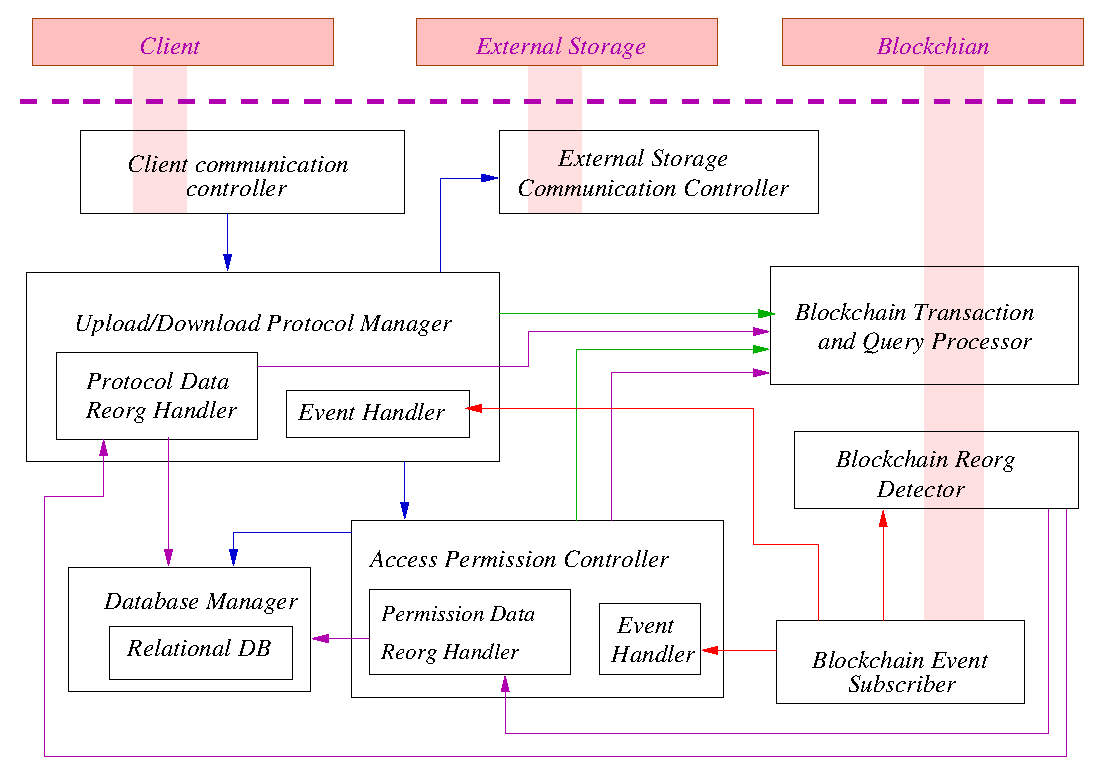
\includegraphics[width=0.48\textwidth]{gateway-design}                    
\caption{Component Breakdown of the Storage Integration Gateway}\label{fig:gatew}
\end{figure}

There are three modules in the gateway for interacting with the blockchain network. {\it Blockchain Transaction and Query Processor} is used during the execution of upload/download protocol for both recording protocol step executions and querying information for protocol initiation and user action validation. Since there may be many gateways in the system that interface the same storage system, protocol transactions issued by a gateway should propagate to others if being mined into blocks. This is achieved by ensuring that any relevant smart contract execution emits events with proper information in the blockchain audit log. The {\it Blockchain Event Subscriber} modules of other gateways capture these events and notify an {\it Event Handler} in their respective {\it Upload/download Protocol Manager} that does database synchronization. Any external action that might change users' access permissions is captured and processed in a similar manner in another blockchain {\it Event Handler} within the {\it Access Permission Controller}.

The gateway issues transactions and receives event notifications by maintaining a connection with some reliable nodes of the blockchain network. At any time, blockchain ledger reorganization can happen in these nodes that may migrate the gateway's transactions to other blocks or throw them away altogether. The gateway must be vigilant and take proper corrective actions in case of such blockchain  reorganizations.

To facilitate proper handling of blockchain reorganization, the gateway retains information about all internal steps of upload and download protocols even after their termination. This information is stored in the gateway database tagged with the hashes (unique block identifiers) of the blocks that recorded the transactions associated with the steps. Similarly, all database entries related to access permission control are also tagged with appropriate block hashes.

If a blockchain reorganization takes place in the nodes the gateway connected with then it becomes aware of the situation through the {\it Blockchain Reorg Detector} module. The module also computes the extent of the reorganization by identifying the blocks that have been dropped in the network. With this information, it initiates two {\it Reorg Handlers} for correcting  upload/download protocol states and for access permission information update. Each {\it Reorg Handler} first retrieves information associated with the blocks from the local database, then searches for their replacement locations in new blocks that caused the chain reorg, and finally determines how to rollback or update the database to bring it to a state consistent with the current version of the blockchain ledger. This database restoration process often involves redoing several transactions in the new blockchain and information update in the external document storage. The underlying algorithm varies with the type of information that is the target of restoration. The process is typically computationally costly and time consuming.                  
       
